\documentclass[]{../util/ColumbiaAssm}

\usepackage{../util/W4400Student}

  \def\mean#1{\mbox{E}\left[ #1 \right]}
\def\var#1{\mbox{Var}\left[ #1 \right]}
\def\cov#1{\mbox{Cov}\left[ #1 \right]}
\def\cmean[#1]#2{\mbox{E}_{#1}\left[ #2 \right]}
\def\skew#1{\mbox{Skew}\left[ #1 \right]}
\def\kurt#1{\mbox{Kurt}\left[ #1 \right]}
\def\Prob#1{\mbox{Pr}\lbrace #1 \rbrace}
\def\cProb[#1]#2{\mbox{Pr}_{#1}\lbrace #2\rbrace}
\def\Pmass#1{P\left( #1 \right)}
\def\Pdens#1{p\left( #1 \right)}
\def\iid{i.~i.~d.\ }
\def\Iid{I.~i.~d.\ }
\def\argmax#1{\textrm{arg}\max_{#1}}
\def\argmin#1{\textrm{arg}\min_{#1}}
\def\kld#1{D_{\mbox{\tiny KL}}\left( #1 \right)}
\def\hist{\mathbf{h}}
\def\entropy#1{H\lbrack #1 \rbrack}
\def\nBins{N_{\mbox{\tiny bins}}}
\newcommand{\bs}[1]{\boldsymbol{#1}}


%%%% FOR EXAM PACKAGE
\printanswers % If you don't want to print answers
\addpoints % if you want to count the points
% \noaddpoints % if you don't want to count the points
% Specifies the way question are displayed:
%\qformat{\textbf{Question \thequestion}\quad(\thepoints)\hfill}
%\qformat{Question \thequestion:\hfill }
\qformat{\thequestion. \textbf{\thequestiontitle} (\thepoints)\hfill }
\usepackage{color} % defines a new color
\definecolor{SolutionColor}{rgb}{0.1,0.1,0.1} % light blue
%\shadedsolutions % defines the style of the solution environment
\framedsolutions % defines the style of the solution environment
% Defines the title of the solution environment:
\renewcommand{\solutiontitle}{\noindent\emph{Solution:~~~}\noindent}
\usepackage{epstopdf}

\usepackage{latexsym}
\usepackage{amsmath,amsfonts,amssymb}
\usepackage{epic}
\usepackage{eepic}
\usepackage{epsfig}
\usepackage{listings}
\usepackage{enumitem}
\usepackage{graphicx}

\begin{document}
  \makeAssmHeader{2}{Due: Tuesday 23 February 2016}
  \vspace{-2cm}

\AddSubmissionRules


  \vspace{0.5cm}

  \def\Rd{\mathbb{R}^d}
  \def\indH{\mbox{\tiny H}}
  \def\v{\mathbf{v}}
  \def\sign{\mbox{sgn}}
  \def\sp#1{\left< #1\right>}
  \def\train{\tilde{\x}}
  \def\trainlabel{\tilde{y}}
  \def\x{\mathbf{x}}
  \def\y{\mathbf{y}}
  \def\z{\mathbf{z}}


\begin{questions}


%%%%%%%%%%%%%%%%%%%%%%%%%%%%
\titledquestion{Linear Classification}[20]
   
   \def\indH{\mbox{\tiny H}}
Consider a perceptron classifier in $\mathbb{R}^2$, given by a hyperplane with orthogonal vector $v_{\indH}$ and offset $c$, and two points
$\mathbf{x}_1$ and $\mathbf{x}_2$. Suppose that
\begin{equation*}
  v_{\indH}:=\left(\begin{matrix}\frac{1}{\sqrt{2}}\\\frac{1}{\sqrt{2}}\end{matrix}\right)
  \qquad
  c:=\frac{1}{2\sqrt{2}}
  \qquad
  \mathbf{x}_1:=\left(\begin{matrix}-3\\0\end{matrix}\right)
    \qquad
    \mathbf{x}_2:=\left(\begin{matrix}\frac{1}{2}\\\frac{1}{2}\end{matrix}\right) \;.
\end{equation*}
\begin{enumerate}
\item (7 points) Compute the classification result for ${\mathbf{x}_1}$ and
  ${\mathbf{x}_2}$.
\item (7 points) If the classifier is given by the same pair $(v_{\indH},-c)$, but was trained as an SVM with
  margin 1, do the results change? Please explain your answer.
\item (6 points) Which cost function does the perceptron cost function
  approximate, and why do we approximate it?
\end{enumerate}

\begin{solution}\\
1. $\textrm{sgn}(\sp{x_1, v_H} - c) = \textrm{sgn}(\frac{-3}{\sqrt(2)} - \frac{1}{2\sqrt(2)}) = -1$, $\textrm{sgn}(\sp{x_2, v_H} - c) = \textrm{sgn}(\frac{2}{2\sqrt(2)} - \frac{1}{2\sqrt(2)}) = 1$\\
2. Since $\sp{x_1, v_H} - c = \frac{-3}{\sqrt(2)} - \frac{1}{2\sqrt(2)} = \frac{-7}{2\sqrt(2)} = -2.82 < -1$, $x_1$ will be classified as -1. However, $\sp{x_2, v_H} - c = \frac{2}{2\sqrt(2)} - \frac{1}{2\sqrt(2)} = \frac{1}{2\sqrt(2))} < 1$, $x_2$ would fall within the 1 margin and would not be classified.\\
3. The perceptron cost function approximates the empirical risk which is piece-wise constant function. As such a function is not suitable for numerical optimisation, we approximate the empirical risk with a piece-wise linear function instead to enable gradient descent.
\end{solution}
%%%%%%%%%%%%%%%%%%%%%%%%%%%%

%%%%%%%%%%%%%%%%%%%%%%%%%%%%
\titledquestion{Perceptron}[40]

%%TITLE: The Perceptron.
%%
Our Perceptron implementation will use the homogeneous coordinate
representation of vectors, i.e.~vectors $\mathbf{x}\in\mathbb{R}^d$ are
represented by $(\mathbf{x},1)=\left( x_1,\dots,x_d,1\right)^t\in\mathbb{R}^{d+1}$.
Recall that this representation turns affine hyperplanes 
\def\vH{\mathbf{v}_{\mbox{\tiny H}}}
\def\zH{\mathbf{z}_{\mbox{\tiny H}}}
\def\sp#1{\left<#1\right>}
\begin{equation*}
        \lbrace
\mathbf{x}\in\mathbb{R}^{d} | \sp{\vH,\mathbf{x})} -c = 0
\rbrace
\end{equation*}
with normal vector $\vH=\left(v_1,\dots,v_d\right)^t$
into hyperplanes through the origin of the form
\begin{equation*}
\lbrace
(\mathbf{x},1)\in\mathbb{R}^{d+1} |
\left(\vH,-c\right)^t (\mathbf{x},1)=0
\rbrace\;.
\end{equation*}

To work with a Perceptron, we need a two-class set of linearly
separable data. For the purposes of testing the algorithm, we will random-generate
this data synthetically. A sample set of $n$ data values
in $d$-dimensional space will be represented
as a $n\times\left( d + 1\right)$-matrix {\tt S}, so each
row is the (homogeneous coordinate) representation of a single
data point. This matrix contains the data of both classes, so in
addition, we need class labels. Class labels are represented
as a vector {\tt y} of length $n$, with entries in $\lbrace -1,+1 \rbrace$.

This problem requires linearly separable data. You can download the function
{\tt fakedata.R} from the class homepage, which generates such data synthetically:
If {\tt z} is a the vector $(\vH,-c)$ and {\tt n} the size of the training data set,
{\tt fakedata(z, n)} returns the matrix {\tt S} and the class label vector {\tt y}.
(Alternatively, you can also write your own implementation of {\tt fakedata}, if you are so inclined---any function that generates linearly separable, Euclidean data is fine.)

\vspace{0.5cm}

\textbf{Homework questions:}
\begin{enumerate}
\item (10 points) To evaluate a Perceptron solution (a hyperplane
  classifier trained by a Perceptron algorithm), write a function
  {\tt classify(S,z)} (where $z=(v,-c)$ is the vector defining the hyperplane) 
  and return class label vector {\tt y} as described above. {\tt S} is a sample data set and {\tt v}
  the Perceptron weight vector (which will be returned by the
  Perceptron training algorithm). 
\item (10 points) Implement the Perceptron training algorithm (see slide 38) with 
    ${\alpha\left( k\right) = \frac{1}{k}}$,
    where $k$ is the number of the current
    iteration. The training algorithm should be an R function 
    {\tt perceptrain(S,y)} which returns a list containing {\tt z} and {\tt Z\_history},
    where ${\tt z}$ is again the normal vector $\zH$ of the hyperplane.
    {\tt Z\_history} is a matrix containing the history
    of the normal vector throughout the training run, i.e.\ a 
    $\left(\mbox{number of iterations}\right)\times\left( d+1\right)$
    matrix, the rows of which are the interim results for {\tt z}.
    
  A recommended sanity check is to train your
  {\tt perceptron} function on a {\tt fakedata} sample, and to make
  sure that the classifier returned by your Perceptron algorithm
  correctly classifies its own training data.
\item (10 points) Generate a new 3D random vector {\tt z}, run {\tt
  fakedata(z,100)}, and train your Perceptron on this
  set. Re-run 
  {\tt fakedata} with the same {\tt z} to produce a test set, and check whether
  it is classified correctly.
\item (10 points) Convert the data and the vectors into their corresponding 2D representation to
  make it more suitable for plotting.
\end{enumerate}
As a solution, please submit:
\begin{itemize}
\item \textbf{all} your program code.
\item One plot showing the test data set and the classifier
  hyperplane, and one showing the training data and the trajectory of the algorithm by
  visualizing {\tt Z\_history}.
  \end{itemize}    

%
% Peter Orbanz, 2006
% modified by chrsigg, 2007
% modified by jpc 2014
%


\begin{solution}
\\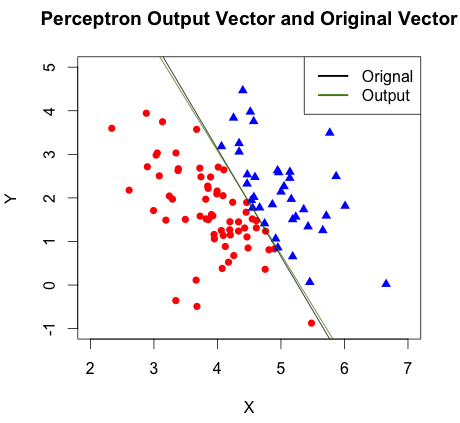
\includegraphics[scale=0.725]{PVvsOV}
\\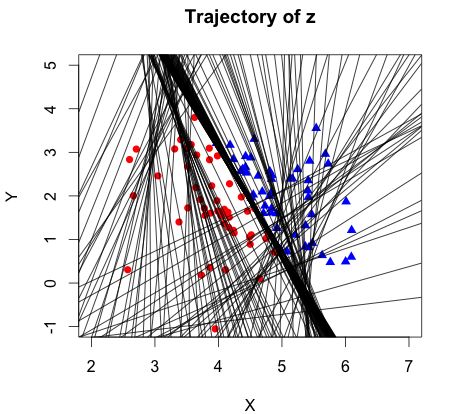
\includegraphics[scale=0.725]{TraZ}
\end{solution}
%%%%%%%%%%%%%%%%%%%%%%%%%%%%

%%%%%%%%%%%%%%%%%%%%%%%%%%%%
\titledquestion{SVM}[40]

%
% Titel: Support vector machines in R
%

In this problem, we will apply a support vector machine to classify hand-written digits. You do not have to implement the SVM algorithm: 
The R library e1071 provides an implementation, see

{\tt http://cran.r-project.org/web/packages/e1071/index.html}

\begin{minipage}{0.7\textwidth}
Download the digit data set from the course website. The zip archive contains two files: Both files are text files. The file
{\tt uspsdata.txt} contains a matrix with one data point (= vector of length 256) per row. 
The 256-vector in each row represents a $16\times 16$ 
image of a handwritten number. The file {\tt uspscl.txt} contains the corresponding class labels. 
The data contains two classes---the digits 5 and 6---so the class labels are stored as -1 and +1, respectively.
The image on the right shows the first row, re-arranged as a $16\times 16$ matrix and plotted as a gray scale image.
\end{minipage}
\begin{minipage}{0.3\textwidth}
  \begin{center}
  
\includegraphics[width=3cm]{usps_digit_example.png}
  \end{center}
\end{minipage}

\begin{itemize}
\item Randomly select about $20\%$ of the data and set it aside as a test set.
\item Train a linear SVM with soft margin. Cross-validate the margin parameter.
\item Train an SVM with soft margin and RBF kernel. You will have to cross-validate both the soft-margin parameter and the kernel bandwidth.
\item After you have selected parameter values for both algorithms, train each one with the parameter value you have chosen. Then
  compute the misclassification rate (the proportion of misclassified data points) on the test set.
\end{itemize}
\textbf{Homework questions:}
\begin{enumerate}
\item (20 points) Plot the cross-validation estimates of the misclassification
rate. Please plot the rate as
  \begin{enumerate}
  \item a function of the margin parameter in the linear case.
  \item a function of the margin parameter and the kernel bandwidth in the non-linear case.
  \end{enumerate}
\item (20 points) Report the test set estimates of the misclassification rates for both cases, with the parameter values you have selected, and
  compare the two results. Is a linear SVM a good choice for this data, or should we use a non-linear one?
%% \item Your experiments may produce a few misclassified
%%   samples---if not, just note that in your homework solution. 
%%   If there are misclassified examples, please plot up to five of these images like the
%%   one above. To do so, you will have to write a 
%%   256-vector into a 16x16 matrix and plot this matrix as an image.
%%   Can you see a qualitative difference between correctly classified and misclassified digits?
\end{enumerate}

Again, in addition to the above, please submit \textbf{all} your program code.


%% \begin{enumerate}
%% \item Randomly select $20\%$ of the data and put it aside as a test set.
%% \item Train a linear SVM with soft margin. Cross-validate the margin parameter.
%% \item Train an SVM with soft margin and RBF kernel. You will have to cross-validate both the soft-margin parameter and the kernel bandwidth.
%% \item After you have selected parameter values for both algorithms, train each one with the optimal parameter value. Then
%%   compute the misclassification rate (the proportion of misclassified data points) on the test set.
%% \item For each method (linear and RBF), select five correctly and five incorrectly classified samples.
%%   Plot these as images like the one above. To do so, you will have to write a 256-vector into a 16x16 matrix and plot this matrix as an image.
%%   Can you see a qualitative difference between correctly classified and misclassified digits?
%% \end{enumerate}


\begin{solution}
\\1a) and 1b) For 1b, the best four combinations of parameters are plotted.
\\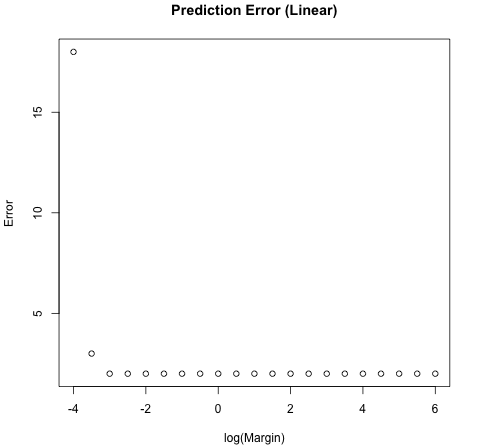
\includegraphics[scale=0.7]{Err_Lin}
\\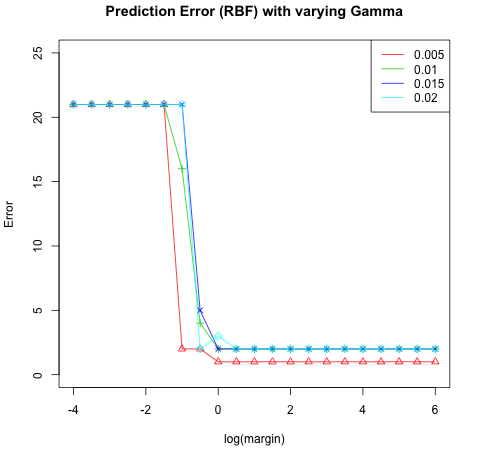
\includegraphics[scale=0.7]{Err_RBF}
\\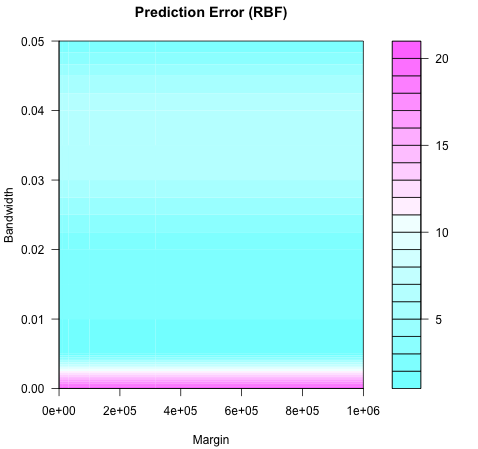
\includegraphics[scale=0.7]{Contour}
\\2 
\begin{lstlisting}
                Test
Linear (0.01)  -1  1
            -1 21  0
            1   2 17

                Test
RBF(100,0.005) -1  1
            -1 21  0
            1   2 17
\end{lstlisting}
Since the result for a linear SVM and a RBF SVM is comparable, we should use a linear SVM as the model is less complex, more interpretable and requires less computation.
\end{solution}
%%%%%%%%%%%%%%%%%%%%%%%%%%%%

%%%%%%%%%%%%%%%%%%%%%%%%%%%%%%%%
\end{questions}
%%%%%%%%%%%%%%%%%%%%%%%%%%%%%%%%

%%%%%%%%%%%%%%%%%%%%%%%%%%%%%%%%
%%%%%%%%%%%%%%%%%%%%%%%%%%%%%%%%
%%%%%%%%%%%%%%%%%%%%%%%%%%%%%%%%
%%%%%%%%%%%%%%%%%%%%%%%%%%%%%%%%
\end{document}
%%%%%%%%%%%%%%%%%%%%%%%%%%%%%%%%
%%%%%%%%%%%%%%%%%%%%%%%%%%%%%%%%
%%%%%%%%%%%%%%%%%%%%%%%%%%%%%%%%
%%%%%%%%%%%%%%%%%%%%%%%%%%%%%%%%
